\documentclass[]{article}
\usepackage{lmodern}
\usepackage{amssymb,amsmath}
\usepackage{ifxetex,ifluatex}
\usepackage{fixltx2e} % provides \textsubscript
\ifnum 0\ifxetex 1\fi\ifluatex 1\fi=0 % if pdftex
  \usepackage[T1]{fontenc}
  \usepackage[utf8]{inputenc}
\else % if luatex or xelatex
  \ifxetex
    \usepackage{mathspec}
  \else
    \usepackage{fontspec}
  \fi
  \defaultfontfeatures{Ligatures=TeX,Scale=MatchLowercase}
\fi
% use upquote if available, for straight quotes in verbatim environments
\IfFileExists{upquote.sty}{\usepackage{upquote}}{}
% use microtype if available
\IfFileExists{microtype.sty}{%
\usepackage{microtype}
\UseMicrotypeSet[protrusion]{basicmath} % disable protrusion for tt fonts
}{}
\usepackage[margin=1in]{geometry}
\usepackage{hyperref}
\hypersetup{unicode=true,
            pdftitle={Evaluación},
            pdfborder={0 0 0},
            breaklinks=true}
\urlstyle{same}  % don't use monospace font for urls
\usepackage{color}
\usepackage{fancyvrb}
\newcommand{\VerbBar}{|}
\newcommand{\VERB}{\Verb[commandchars=\\\{\}]}
\DefineVerbatimEnvironment{Highlighting}{Verbatim}{commandchars=\\\{\}}
% Add ',fontsize=\small' for more characters per line
\usepackage{framed}
\definecolor{shadecolor}{RGB}{248,248,248}
\newenvironment{Shaded}{\begin{snugshade}}{\end{snugshade}}
\newcommand{\KeywordTok}[1]{\textcolor[rgb]{0.13,0.29,0.53}{\textbf{#1}}}
\newcommand{\DataTypeTok}[1]{\textcolor[rgb]{0.13,0.29,0.53}{#1}}
\newcommand{\DecValTok}[1]{\textcolor[rgb]{0.00,0.00,0.81}{#1}}
\newcommand{\BaseNTok}[1]{\textcolor[rgb]{0.00,0.00,0.81}{#1}}
\newcommand{\FloatTok}[1]{\textcolor[rgb]{0.00,0.00,0.81}{#1}}
\newcommand{\ConstantTok}[1]{\textcolor[rgb]{0.00,0.00,0.00}{#1}}
\newcommand{\CharTok}[1]{\textcolor[rgb]{0.31,0.60,0.02}{#1}}
\newcommand{\SpecialCharTok}[1]{\textcolor[rgb]{0.00,0.00,0.00}{#1}}
\newcommand{\StringTok}[1]{\textcolor[rgb]{0.31,0.60,0.02}{#1}}
\newcommand{\VerbatimStringTok}[1]{\textcolor[rgb]{0.31,0.60,0.02}{#1}}
\newcommand{\SpecialStringTok}[1]{\textcolor[rgb]{0.31,0.60,0.02}{#1}}
\newcommand{\ImportTok}[1]{#1}
\newcommand{\CommentTok}[1]{\textcolor[rgb]{0.56,0.35,0.01}{\textit{#1}}}
\newcommand{\DocumentationTok}[1]{\textcolor[rgb]{0.56,0.35,0.01}{\textbf{\textit{#1}}}}
\newcommand{\AnnotationTok}[1]{\textcolor[rgb]{0.56,0.35,0.01}{\textbf{\textit{#1}}}}
\newcommand{\CommentVarTok}[1]{\textcolor[rgb]{0.56,0.35,0.01}{\textbf{\textit{#1}}}}
\newcommand{\OtherTok}[1]{\textcolor[rgb]{0.56,0.35,0.01}{#1}}
\newcommand{\FunctionTok}[1]{\textcolor[rgb]{0.00,0.00,0.00}{#1}}
\newcommand{\VariableTok}[1]{\textcolor[rgb]{0.00,0.00,0.00}{#1}}
\newcommand{\ControlFlowTok}[1]{\textcolor[rgb]{0.13,0.29,0.53}{\textbf{#1}}}
\newcommand{\OperatorTok}[1]{\textcolor[rgb]{0.81,0.36,0.00}{\textbf{#1}}}
\newcommand{\BuiltInTok}[1]{#1}
\newcommand{\ExtensionTok}[1]{#1}
\newcommand{\PreprocessorTok}[1]{\textcolor[rgb]{0.56,0.35,0.01}{\textit{#1}}}
\newcommand{\AttributeTok}[1]{\textcolor[rgb]{0.77,0.63,0.00}{#1}}
\newcommand{\RegionMarkerTok}[1]{#1}
\newcommand{\InformationTok}[1]{\textcolor[rgb]{0.56,0.35,0.01}{\textbf{\textit{#1}}}}
\newcommand{\WarningTok}[1]{\textcolor[rgb]{0.56,0.35,0.01}{\textbf{\textit{#1}}}}
\newcommand{\AlertTok}[1]{\textcolor[rgb]{0.94,0.16,0.16}{#1}}
\newcommand{\ErrorTok}[1]{\textcolor[rgb]{0.64,0.00,0.00}{\textbf{#1}}}
\newcommand{\NormalTok}[1]{#1}
\usepackage{graphicx,grffile}
\makeatletter
\def\maxwidth{\ifdim\Gin@nat@width>\linewidth\linewidth\else\Gin@nat@width\fi}
\def\maxheight{\ifdim\Gin@nat@height>\textheight\textheight\else\Gin@nat@height\fi}
\makeatother
% Scale images if necessary, so that they will not overflow the page
% margins by default, and it is still possible to overwrite the defaults
% using explicit options in \includegraphics[width, height, ...]{}
\setkeys{Gin}{width=\maxwidth,height=\maxheight,keepaspectratio}
\IfFileExists{parskip.sty}{%
\usepackage{parskip}
}{% else
\setlength{\parindent}{0pt}
\setlength{\parskip}{6pt plus 2pt minus 1pt}
}
\setlength{\emergencystretch}{3em}  % prevent overfull lines
\providecommand{\tightlist}{%
  \setlength{\itemsep}{0pt}\setlength{\parskip}{0pt}}
\setcounter{secnumdepth}{0}
% Redefines (sub)paragraphs to behave more like sections
\ifx\paragraph\undefined\else
\let\oldparagraph\paragraph
\renewcommand{\paragraph}[1]{\oldparagraph{#1}\mbox{}}
\fi
\ifx\subparagraph\undefined\else
\let\oldsubparagraph\subparagraph
\renewcommand{\subparagraph}[1]{\oldsubparagraph{#1}\mbox{}}
\fi

%%% Use protect on footnotes to avoid problems with footnotes in titles
\let\rmarkdownfootnote\footnote%
\def\footnote{\protect\rmarkdownfootnote}

%%% Change title format to be more compact
\usepackage{titling}

% Create subtitle command for use in maketitle
\newcommand{\subtitle}[1]{
  \posttitle{
    \begin{center}\large#1\end{center}
    }
}

\setlength{\droptitle}{-2em}

  \title{Evaluación}
    \pretitle{\vspace{\droptitle}\centering\huge}
  \posttitle{\par}
    \author{}
    \preauthor{}\postauthor{}
    \date{}
    \predate{}\postdate{}
  

\begin{document}
\maketitle

\subsection{Consideraciones}\label{consideraciones}

\begin{itemize}
\tightlist
\item
  Para esta evaluación usted debera entregar un script de R con los
  comandos necesarios para responder cada uno de los puntos.
\item
  Además se evaluará la calidad (no necesariamente la cantidad) de
  comentarios en las respuestas.
\item
  Esta evaluación se puede hacer en grupo de máximo 3 personas.
\item
  La forma de entrega será vía email a
  \textbf{\href{mailto:jbkunst@gmail.com}{\nolinkurl{jbkunst@gmail.com}}}
  con plazo el día viernes 7 de diciembre.
\end{itemize}

\subsection{Ejericicio 1}\label{ejericicio-1}

Considere los siguientes datos de alumnos encuestados al final de
semestre sobre un curso de R:

\begin{Shaded}
\begin{Highlighting}[]
\KeywordTok{library}\NormalTok{(tidyverse)}

\NormalTok{alumnos <-}\StringTok{ }\KeywordTok{read_csv}\NormalTok{(}\StringTok{"https://goo.gl/Wy3GsU"}\NormalTok{)}
\KeywordTok{glimpse}\NormalTok{(alumnos)}
\end{Highlighting}
\end{Shaded}

\begin{verbatim}
## Observations: 3,000
## Variables: 3
## $ dificultad   <dbl> 39.64, 50.66, 36.79, 69.86, 52.64, 37.00, 54.79, ...
## $ satisfaccion <dbl> 62.78, 57.49, 67.23, 44.47, 43.84, 64.77, 65.74, ...
## $ grupo        <chr> "grp04", "grp03", "grp04", "grp02", "grp02", "grp...
\end{verbatim}

A cada alumno encuestado se le preguntó sobre su satisfacción y
percepción de la duración del curso.

\begin{itemize}
\tightlist
\item
  Obtenga un diagrama de puntos entre las variables \texttt{duracion} y
  \texttt{satisfaccion}.
\item
  Comente respecto al resultado. Intente realizar una hipótesis respecto
  a lo que observa.
\item
  Al gráfico anterior agregue una línea de tendencia usando la funcion
  \texttt{geom\_smooth} (Puede revisar ejemplos, ejecutar
  \texttt{?geom\_smooth})
\end{itemize}

Ahora suponga que el equipo académico le recomienda considerar el grupo
de donde el alumno proviene para así seguir estudiando la evidencia
encontrada en el punto anterior:

\begin{itemize}
\tightlist
\item
  Vuelva a hacer un diagrama de puntos pero ahora diferenciando mediante
  el color al grupo al que el alumno pertenece.
\item
  Al grafico anterior agregue una línea de tendendencia y además utilice
  el comando \texttt{facet\_wrap} para crear graficos de acuerdo al
  grupo del alumno.
\item
  Con lo obtenido, ¿Qué sucede con la hipótesis obtenida anteriormente?
\end{itemize}

\subsection{Ejercicio 2}\label{ejercicio-2}

En esta parte trabajaremos con datos de variaciones de temperatura
durante los años:

\begin{Shaded}
\begin{Highlighting}[]
\NormalTok{temperatura <-}\StringTok{ }\KeywordTok{read_csv}\NormalTok{(}\StringTok{"https://goo.gl/3JUCma"}\NormalTok{)}
\NormalTok{temperatura}
\end{Highlighting}
\end{Shaded}

\begin{verbatim}
## # A tibble: 1,992 x 5
##    anio_mes   mediana inferio superio decada
##    <date>       <dbl>   <dbl>   <dbl>  <int>
##  1 1850-01-01  -0.702  -1.10   -0.299   1850
##  2 1850-02-01  -0.281  -0.673   0.117   1850
##  3 1850-03-01  -0.732  -1.08   -0.382   1850
##  4 1850-04-01  -0.569  -0.904  -0.237   1850
##  5 1850-05-01  -0.326  -0.662   0.005   1850
##  6 1850-06-01  -0.212  -0.515   0.085   1850
##  7 1850-07-01  -0.128  -0.457   0.199   1850
##  8 1850-08-01  -0.232  -0.595   0.132   1850
##  9 1850-09-01  -0.435  -0.808  -0.063   1850
## 10 1850-10-01  -0.452  -0.793  -0.104   1850
## # ... with 1,982 more rows
\end{verbatim}

\begin{itemize}
\tightlist
\item
  Relice un gráfico de línea considerando las columnas
  \texttt{anio\_mes} y \texttt{mediana}
\item
  Ahora cargue el paquete \texttt{lubridate}, y usando las funciones
  \texttt{year} y \texttt{month} sobre la columna \texttt{anio\_mes}
  cree dos variables en la tabla \texttt{temperatura} y nómbrelas como
  \texttt{anio} y \texttt{mes}.
\item
  Revise y considere los ejemplo de \texttt{geom\_raster} (intente
  ejecutar \texttt{?geom\_raster}) para usarlo con los datos de
  \texttt{anio}, \texttt{mes} y \texttt{mediana} y comenta que observas.
\item
  Agrupe la tabla temperatura usando la columna \texttt{anio} para
  obtener el promedio de la columna \texttt{mediana}.
\item
  Con lo anterior vuelva a obtener un grafico del promedio obtenido
  anteriormente por año.
\item
  Si tuviese que escoger alguna de las dos alternativas de gráficos de
  líneas para presentarla a alguién que nuevo en el tema, ¿Cual
  escogería y por que?
\end{itemize}

\subsection{Ejercicio 3}\label{ejercicio-3}

Trabajaremos con los siguientes datos utilizados anteriormente:

\begin{Shaded}
\begin{Highlighting}[]
\NormalTok{miembros <-}\StringTok{ }\KeywordTok{read_csv}\NormalTok{(}\StringTok{"https://goo.gl/Tigfaj"}\NormalTok{)}
\KeywordTok{glimpse}\NormalTok{(miembros)}
\end{Highlighting}
\end{Shaded}

\begin{verbatim}
## Observations: 83
## Variables: 3
## $ funcion      <chr> "analista", "analista", "analista", "analista", "...
## $ nombre       <chr> "Alberto Recarte Garcia Andrade", "Alejandro Couc...
## $ organizacion <chr> "banco", "consultora", "banco", "banco", "banco",...
\end{verbatim}

\begin{Shaded}
\begin{Highlighting}[]
\NormalTok{movimientos <-}\StringTok{ }\KeywordTok{read_csv}\NormalTok{(}\StringTok{"https://goo.gl/fT3jwT"}\NormalTok{)}
\KeywordTok{glimpse}\NormalTok{(movimientos)}
\end{Highlighting}
\end{Shaded}

\begin{verbatim}
## Observations: 77,202
## Variables: 8
## $ nombre             <chr> "Alberto Recarte Garcia Andrade", "Alberto ...
## $ fecha              <chr> "2003-01-03 23:00:00 UTC", "2003-01-03 23:0...
## $ hora               <int> 12, 12, 19, 15, 16, 15, 10, 12, 15, 15, 15,...
## $ minuto             <int> 30, 32, 7, 31, 5, 27, 20, 58, 25, 28, 28, 2...
## $ importe            <dbl> 38.70, 14.60, 95.62, 49.13, 13.94, 80.00, 5...
## $ comercio           <chr> "RCG OFICINA", "MANZANIL AREA", "REST REAL ...
## $ actividad_completa <chr> "CONFECCION TEXTIL EN GENERAL", "HOTELES,MO...
## $ actividad          <chr> "ROPA", "HOTEL", "RESTAURANTE", "COCHE", "C...
\end{verbatim}

Con la función \texttt{ymd\_hms} del paquete \texttt{lubridate} puede
\emph{parsear} (convertir) la columna fecha (que es texto!) a
fecha-hora. Luego con la función \texttt{as.Date} puedes tranformar el
campo de fecha-hora a fecha.

\begin{itemize}
\tightlist
\item
  Con lo anterior agrupe por dias y obtenga el número de operaciones,
  como también el importe total por día de la tabla
  \texttt{movimientos}.
\item
  Grafique, de forma separada estas dos variables (por fecha). ¿Qué tipo
  de \texttt{geom\_} puede ser opción?
\item
  Obtenga la suma de los importes por actividad de los miembros
\item
  Con la tabla anterior grafíquelos usando \texttt{geom\_col}.
\item
  Obtenga la suma de los importes por actividad y hora, luego utilice
  \texttt{geom\_tile} para mostrar la información obtenida y comente.
\item
  ¿Que es lo que muestra el siguiente gráfico, y que podría hacer con
  esta información en el caso que usted sea?
\end{itemize}

\begin{Shaded}
\begin{Highlighting}[]
\KeywordTok{library}\NormalTok{(tidyverse)}

\KeywordTok{ggplot}\NormalTok{(movimientos) }\OperatorTok{+}
\StringTok{  }\KeywordTok{geom_point}\NormalTok{(}\KeywordTok{aes}\NormalTok{(importe, actividad), }\DataTypeTok{alpha =} \FloatTok{0.5}\NormalTok{)}
\end{Highlighting}
\end{Shaded}

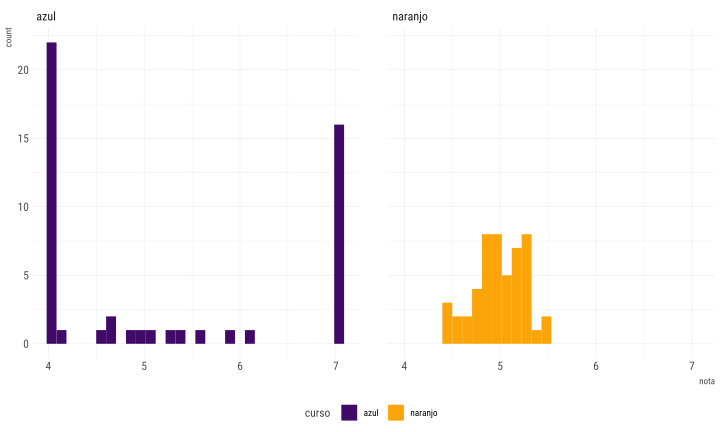
\includegraphics{09-evaluación_files/figure-latex/unnamed-chunk-4-1.pdf}

\begin{itemize}
\tightlist
\item
  Usando la imagen anterior identifique usted 3 casos
  (puntos/movimientos) que le llamen la atentción y descríbalos:
  Describiendo la hora, quien realizó la operación, el monto, la
  actividad, etc, y comente si el dato parece digno de investigar o no.
\end{itemize}


\end{document}
